\begin{figure}[t]
\begin{center}
\centerline{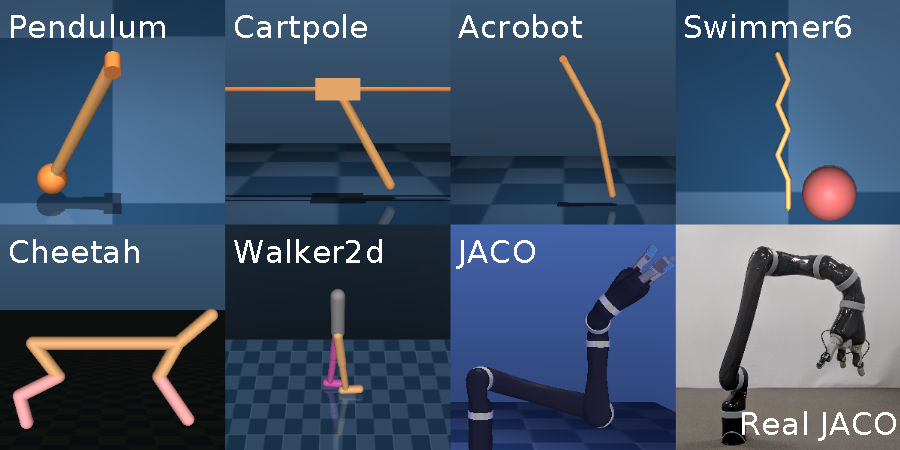
\includegraphics[width=\columnwidth]{figures/environments}}\vspace{0.2cm}\centerline{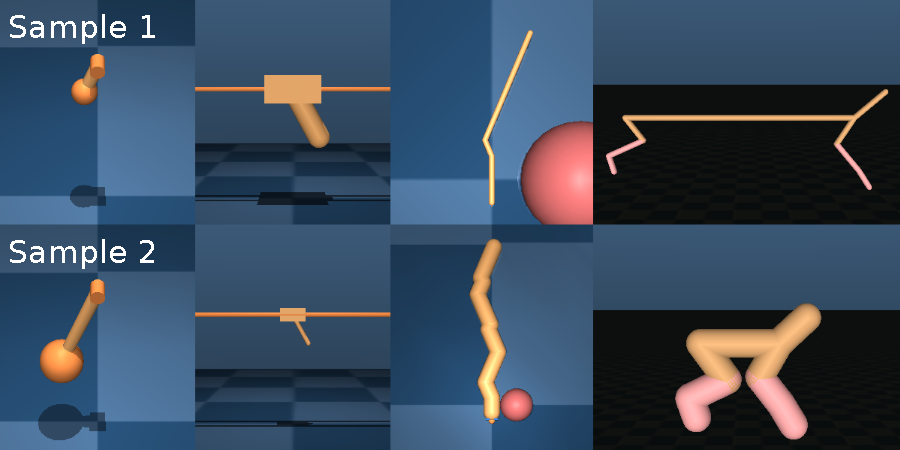
\includegraphics[width=\columnwidth]{figures/environment_parametrizations}}
\vspace{-0.1in}
\caption{(Top) Our experimental physical systems. (Bottom) Samples of parametrized versions of these systems (see videos: \href{\environmentrandomtrajectories}{link}). 
}
\label{fig:environments}
\end{center}
\vskip -0.2in
\end{figure}